\documentclass[11pt]{article}
\usepackage{bookmark}
\usepackage{algorithm}
\usepackage{algpseudocode}
\usepackage{amsfonts}
\usepackage{amsmath}
\usepackage{amssymb}
\usepackage{amsthm}
\usepackage{bm}
\usepackage{color}
\usepackage{comment}
\usepackage{float}
\usepackage{graphicx}
%\usepackage[hidelinks]{hyperref}
\usepackage{makecell}
\usepackage[caption=false,font=footnotesize,subrefformat=parens,labelformat=parens]{subfig}
\usepackage{wrapfig}
\usepackage{url}
\usepackage[table]{xcolor}
\graphicspath{{images/}}
\setlength{\parindent}{0.25in}
\setlength{\parskip}{.05in}
\pagestyle{plain}
%Title, date an author of the document
\title{Progress Report}
\author{Bardia Mojra}


\begin{document}
\maketitle
\thispagestyle{empty}

\bigskip
\bigskip
\begin{center}
 Robotic Vision Lab
\end{center}

\begin{center}
The University of Texas at Arlington
\end{center}

\newpage

\section{Specific Research Goals}
\begin{itemize}
      \item VPQEKF (\textcolor{red}{April 13th}): Work on the paper.
      \item DLO Manipulation Dataset (ICRA - \textcolor{red}{Sept. 1st})
\end{itemize}

\section{To Do}
\begin{itemize}
  \item QEKF Paper - 30\% extension (\textcolor{red}{April 13th}):
  \begin{itemize}
      \item Edit VEst section and add updates.
  \end{itemize}
  \item QEKF/QuEst+VEst Implementation (\textcolor{red}{April 13th}):
  \begin{itemize}
      \item Implement and test QEKF in Matlab. Done.
      \item OOP Integration: QEKF is done, QuEst is done but not tested, and
VEst is remaining.
      \item Feature point extraction: implement semantic segmentation
      \item Address scale factor (depth-scale) issues: DL solutions?
      \item Address "hand off" issue when objects enter or leave field of view
      \item Real-time streaming images for real-time operation (optional)
      \item Experiments
      \item Noise issue: noise cannot be modeled - revisit
  \end{itemize}
  \item  DLO Manipulation:  \textcolor{red}{Sept. 1st}
  \begin{itemize}
      \item Related work literature review
      \item Real dataset + paper (ICRA -  \textcolor{red}{Sept. 1st}):
      \begin{itemize}
            \item Design, discuss and build a data collection and test rig.
      \end{itemize}
      \item Unity dataset
      \begin{itemize}
            \item Recreate virtual duplicates of physical test material
            \item Model dynamics and deformity
      \end{itemize}
  \end{itemize}
\end{itemize}


\section{Progress}
The following items are listed in the order of priority:
\begin{itemize}
    \item VPQEKF (\textcolor{red}{RAL - April 1st, 2022}): I tested QEKF Matlab
    and shared the results with Dr. Gans. Then, I worked on the
    integration part of the project. To integrate the three modules, I am
    deploying object-oriented programming (OOP) scheme for effective management.
    Everybody writes code, not many write useful code.
    The QEKF module is ready since it is already in OOP format. I finished
    porting in QuEst/main file to OOP format and began testing it. The source code
    has not and will not change since it is implemented in "Static"
    function style (each function in a separate file). Static functions can be
    used as-is in form of local 'scope' functions in Matlab OOP. I have not
    started working on VEst and I estimate it to take less than two days (that
    includes a day for testing). Moreover, the new QuEst code includes all other pose
    estimation methods implemented by Kaveh. The following figure shows my
    contribution to the QEKF project over the past 6 months.

    \begin{figure}
      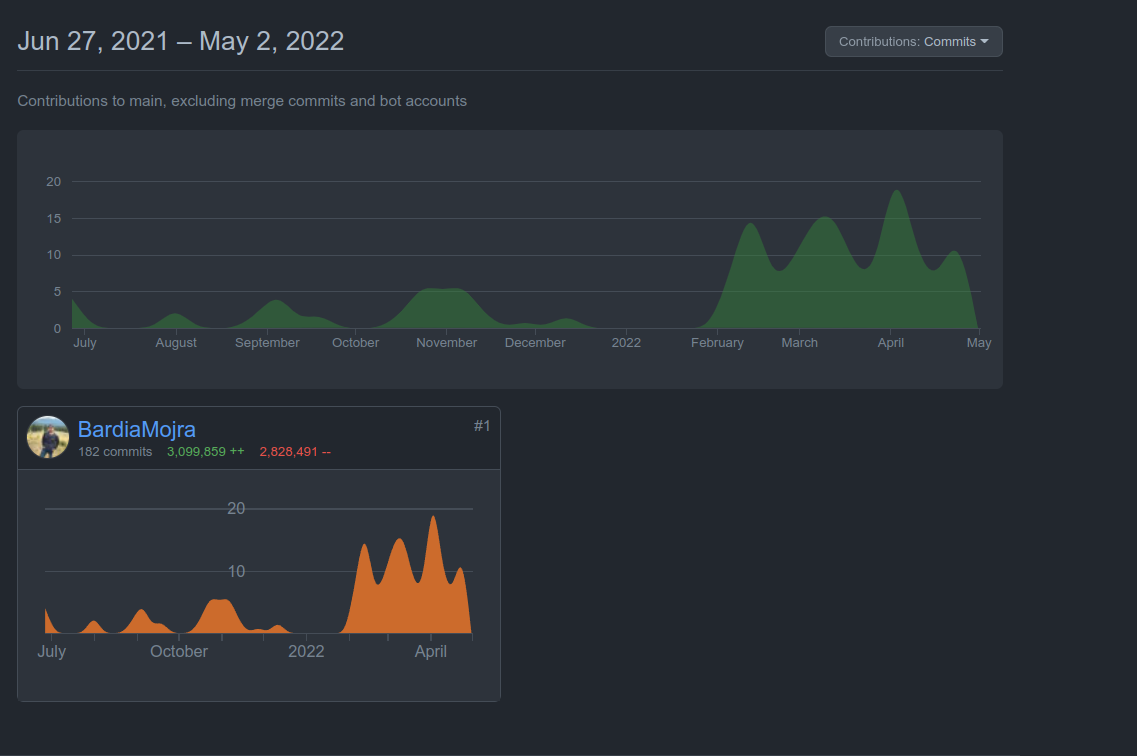
\includegraphics[width=\linewidth]{qekf_contribs.png}
    \end{figure}

    \item DLO Manipulation Milestones: Early in the week, I did some tutorials
    on Blender and began recreating the lab work cell area. Ideally, I will use
    Nvidia's Isaac simulation as I am confident they will use their trade secrets
    to achieve better performance on their hardware compared to all other
    competitors. Moreover, I strongly think adding projectors to the data collection
    rig can significantly improve computer-assisted annotation. The projection
    can be used as closed-loop visual feedback and can be cross-referenced
    with the depth map. You can create robustness by cross-referencing high
    probability estimates. Please don't share this idea with anyone.

    \item 3D Scanner: It is needed for object manipulation and perception tasks.



    \item Pose Estimation (\textcolor{blue}{DLO-01}): On-going under VPQEKF.
    \item Semantic segmentation (\textcolor{blue}{DLO-02}): Per my discussion with Dr. Gans, I
    will explore DL methods for the depth or scale problem.
    \item Grasping Project (\textcolor{blue}{DLO-03}): I am making this a part of the DLO project.
    \item PyTorch Tutorials: Transfer learning.

  \end{itemize}

\section{Intermediate Goals - Fall 2021:}
\begin{itemize}
      \item QEKF: Finish paper.
      \item UR5e: Do the tutorials.
\end{itemize}

\newpage

%Sets the bibliography style to UNSRT and import the
% \newpage
% \bibliography{ref}
% \bibliographystyle{ieeetr}

\end{document}
